\documentclass{article}

\usepackage{graphicx}
\usepackage{float}
\usepackage{caption}
\usepackage{subcaption}
\usepackage{hyperref}

\title{Student job report: Bootstrap high quantiles estimation.}
\author{Joris LIMONIER}
\date{February - May 2021}

\begin{document}
\maketitle

\section{Introduction}
The first analysis took place with the following data

\begin{figure}[H]
    \centering
    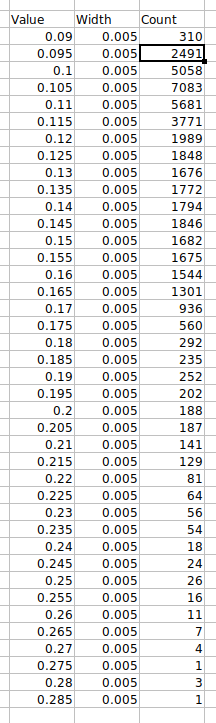
\includegraphics[width=.28\textwidth]{images/excel_data.png}
    \caption{Initial data}
\end{figure}

which can be visually represented as the following histogram

\begin{figure}[H]
    \centering
    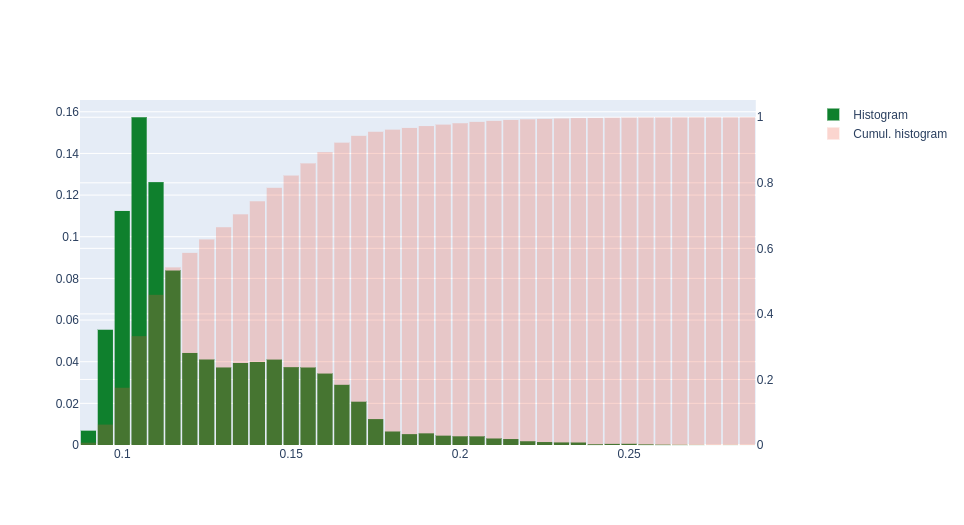
\includegraphics[width=\textwidth]{images/plot_excel_data.png}
    \caption{Visual representation of the initial data}
\end{figure}

We define the n-th quantile as follows:
\begin{equation}
    q_n := 1 - 10^{-n}
\end{equation}
which gives $q_1 = 0.9$, $q_2 = 0.99$ ...etc. Where simply speaking $q_n$ represents 0 followed by $n$ nines. We are mostly interested in $q_3, q_4$ and $q_5$.

\section{Bootstrap}
We use the bootstrap to estimate the value of the quantiles even with small to moderate sample size.

\begin{figure}
    \centering
    \begin{subfigure}{.8 \textwidth}
        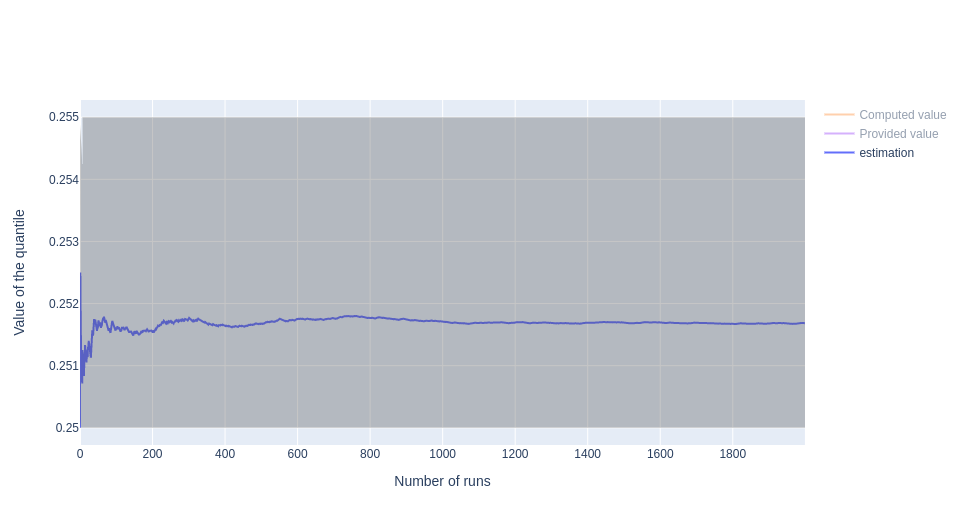
\includegraphics[width=\textwidth]{images/estimation_q3.png}
        \caption{Estimation of $q_3$}
    \end{subfigure}
    \hfill
    \begin{subfigure}{.8 \textwidth}
        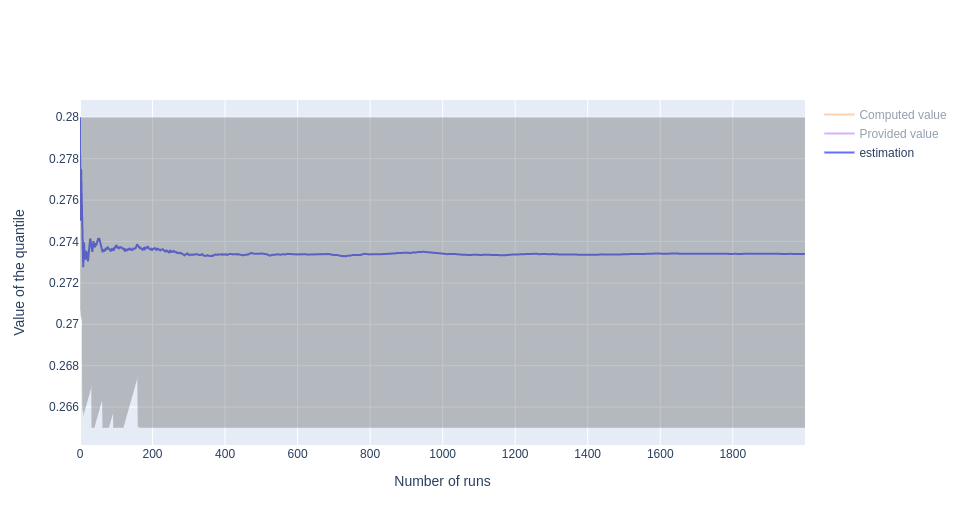
\includegraphics[width=\textwidth]{images/estimation_q4.png}
        \caption{Estimation of $q_4$}
    \end{subfigure}
    \hfill
    \begin{subfigure}{.8 \textwidth}
        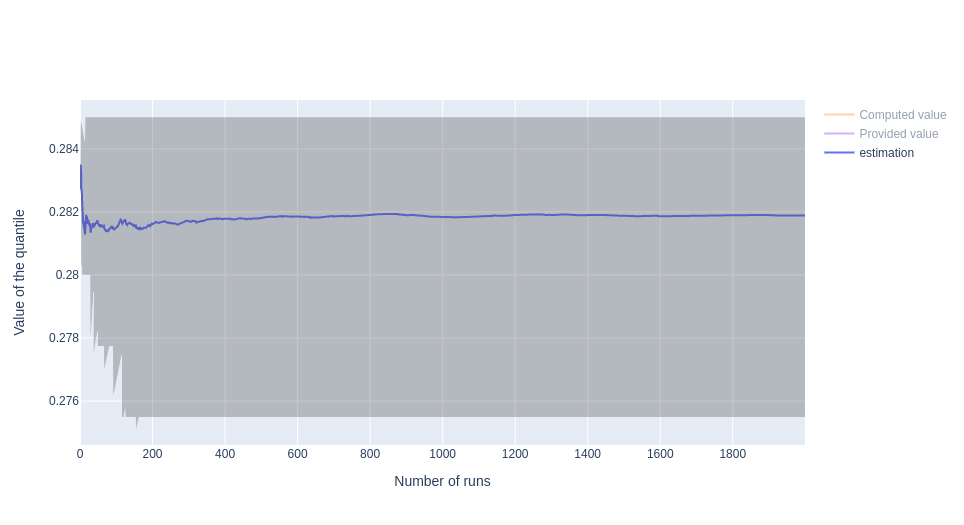
\includegraphics[width=\textwidth]{images/estimation_q5.png}
        \caption{Estimation of $q_5$}
    \end{subfigure}
    \caption{Estimation of the quantiles over bootstrap runs}
    \label{fig: estimation of quantiles}
\end{figure}

The plots in figure \ref{fig: estimation of quantiles} show the evolution of the quantiles as we go through the bootstraps. The grey areas represent the $95\%$ confidence intervals during that evolution.\\
\textbf{According to our data}, it seems that there is close to no change in the estimation of the quantiles after $1000$ repetitions of the bootstrap. The variations are small after 500 runs already but for safety purposes we consider that we have our final guess after 1000 runs. As for the confidence intervals, only in some edge cases do we have changes past the 1000 mark. \\
\textit{NB: We have good empirical evidence to back up our estimate of 1000 runs. It is not a theoretical result, however, we believe that it is suitable for engineering purposes.}

\end{document}